\documentclass{article}
\usepackage[margin=22mm]{geometry}\usepackage{tikz}\usetikzlibrary{positioning}
\begin{document}\section*{Research API boundaries}
Created-at: 2026-10-07T15:43+02:00 (Europe/Budapest). ETA: 60 minutes for API extraction, focused regression and consumer command checks.
\paragraph{Scope} Core remains compilation/IR/identity owner; Query supplies borrowed semantics; Graph owns search and spanning bases; Geometry owns FK/collision; Formats owns domain projections. Binaries own argv, output and campaign scheduling. Simulator retains physical execution. No new engine, crate or dependency version.
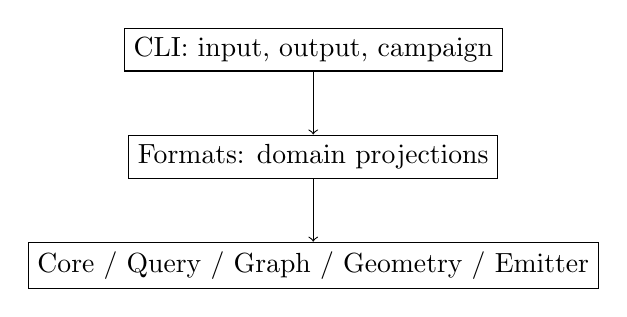
\begin{tikzpicture}[node distance=8mm]\node[draw] (a) {CLI: input, output, campaign};\node[draw,below=of a] (b) {Formats: domain projections};\node[draw,below=of b] (c) {Core / Query / Graph / Geometry / Emitter};\draw[->] (a)--(b);\draw[->] (b)--(c);\end{tikzpicture}
\paragraph{Files} Formats examples adversarial\_grid and four modules, metaheuristic\_contract and profiles, mujoco\_crosscheck; replacement src/environment modules, src/metaheuristic modules, src/robot\_projection.rs and src/bin entries; src/lib.rs, src/codegen.rs, src/transforms.rs, Cargo.toml; Geometry src/transforms/mod.rs; integration tests; retired MJCF templates; Transformation README and shell launcher; Hystl research README; Simulator maze/mission docs if command changes. Generated SYMBOLS and this plan/report.
\paragraph{Interfaces} Library APIs over Core snapshots; preserve schemas, caps, identities, deterministic priorities and output protection. Move existing Graph/Emitter dev dependencies to regular dependencies at unchanged revisions. Remove substantive examples. Route MJCF dispatch to its one existing articulated emitter.
\paragraph{Protected items} None intended. No Simulator manifest or Kawamirai edits. No commits or pushes.
\paragraph{Tests} Before/after existing tests; public API malformed/deterministic regression tests; CLI opt-in tests; scoped Clippy; dependency/duplication audit; Amaterasu fixed DE/GA and hex/polar artifact comparisons. Do not restart the overnight campaign.
\paragraph{Budgets and risks} Preserve 128 KiB source, 4096 declarations, 16x16 grid, 1000 proposals, 8192-byte genome, 64 walls and 32 waypoints. Two compiler workers; no performance campaign. Risks: include paths, visibility, dropped checks, old executable paths, template bypass, unrelated dirty files. Worst input is existing bounded profiles, no scaling claim.
\paragraph{Rollback} Pre-edit snapshots in ignored report artifacts; reverse only task hunks. Preserve historical run evidence and all unrelated work.
\paragraph{Final affected-file inventory} Updated-at: 2026-10-07T16:11+02:00. The consumer audit also identified the existing template-dispatch integration test.\begin{flushleft}\small
\texttt{\detokenize{README.md}}\\
\texttt{\detokenize{hymeko_formats/Cargo.toml}}\\
\texttt{\detokenize{hymeko_formats/examples/adversarial_grid.rs}}\\
\texttt{\detokenize{hymeko_formats/examples/adversarial_grid/maze.rs}}\\
\texttt{\detokenize{hymeko_formats/examples/adversarial_grid/maze_physics.rs}}\\
\texttt{\detokenize{hymeko_formats/examples/adversarial_grid/physical.rs}}\\
\texttt{\detokenize{hymeko_formats/examples/adversarial_grid/visual.rs}}\\
\texttt{\detokenize{hymeko_formats/examples/metaheuristic_contract.rs}}\\
\texttt{\detokenize{hymeko_formats/examples/metaheuristic_contract/profiles.rs}}\\
\texttt{\detokenize{hymeko_formats/examples/mujoco_crosscheck.rs}}\\
\texttt{\detokenize{hymeko_formats/src/bin/adversarial_grid.rs}}\\
\texttt{\detokenize{hymeko_formats/src/bin/adversarial_grid/maze.rs}}\\
\texttt{\detokenize{hymeko_formats/src/bin/metaheuristic_contract.rs}}\\
\texttt{\detokenize{hymeko_formats/src/bin/robot_projection.rs}}\\
\texttt{\detokenize{hymeko_formats/src/codegen.rs}}\\
\texttt{\detokenize{hymeko_formats/src/environment/maze.rs}}\\
\texttt{\detokenize{hymeko_formats/src/environment/maze_physics.rs}}\\
\texttt{\detokenize{hymeko_formats/src/environment/mod.rs}}\\
\texttt{\detokenize{hymeko_formats/src/environment/physical.rs}}\\
\texttt{\detokenize{hymeko_formats/src/environment/visual.rs}}\\
\texttt{\detokenize{hymeko_formats/src/lib.rs}}\\
\texttt{\detokenize{hymeko_formats/src/metaheuristic/mod.rs}}\\
\texttt{\detokenize{hymeko_formats/src/metaheuristic/profiles.rs}}\\
\texttt{\detokenize{hymeko_formats/src/robot_projection.rs}}\\
\texttt{\detokenize{hymeko_formats/src/transforms.rs}}\\
\texttt{\detokenize{hymeko_formats/tests/research_api.rs}}\\
\texttt{\detokenize{hymeko_formats/tools/run_adversarial_grid.sh}}\\
\texttt{\detokenize{hymeko_geometry/src/transforms/mod.rs}}\\
\texttt{\detokenize{hymeko_query/tests/test_template_driven.rs}}\\
\texttt{\detokenize{transforms/mjcf/queries.hymeko}}\\
\texttt{\detokenize{transforms/mjcf/template.mjcf.xml}}\\
\end{flushleft}
\end{document}